\documentclass[10pt, aspectratio=1610]{beamer}
%font setting
\usefonttheme{professionalfonts}
\usepackage[english]{babel}%Language
\usepackage{tikz}%TikZ Picture
\usepackage{amsmath,amssymb,mathtools}%Mathematics
\usepackage{graphicx}% Allows including images
\usepackage{animate}%Allows including gif
\usepackage{multimedia}%Allows including videos
\usepackage{multicol}%Multiple columns in the frame
\usepackage{hyperref}%jump to selected page and return back to the origin
\hypersetup{colorlinks=true, linkcolor=MyBackground}
\usepackage{varioref}
\usepackage{cleveref}
\usepackage[most]{tcolorbox}      
\usepackage{appendix}
\usepackage{environ}% Custom font for a frame.
\newcommand{\customframefont}[1]{
\setbeamertemplate{itemize/enumerate body begin}{#1}
\setbeamertemplate{itemize/enumerate subbody begin}{#1}
}
\NewEnviron{framefont}[1]{
\customframefont{#1} % for itemize/enumerate
{#1 % For the text outside itemize/enumerate
\BODY
}
\customframefont{\normalsize}
}

\definecolor{MyBackground}{rgb}{1.0000,0.9451,0.6549}

\usetheme[block=fill,numbering=fraction,progressbar=frametitle]{metropolis}
\setbeamertemplate{frametitle continuation}{\insertcontinuationcount}
\useoutertheme{metropolis}
\useinnertheme{metropolis}
\usefonttheme{metropolis}

\title{Integration by Parts}
\subtitle{Trial Lecture: A-Level Edexcel Math C4}
\author{Wusheng Zhang}
\date{}
\institute{\large\textbf{Learning Outcome}:\\[6pt] Recognize when to use integration by parts; 
Use the integration-by-parts formula to solve integration problems
}
\everymath{\displaystyle}

\begin{document}
\begin{frame}
\titlepage
\end{frame}

\AtBeginSection[]
{
  \begin{frame}
    \setbeamertemplate{section in toc}[sections numbered]
    \frametitle{Table of Contents}
    \tableofcontents[currentsection]
  \end{frame}
}

\begin{frame}{About Using Software to help you solve exercises}
    \begin{center}
        
\includegraphics[width=0.7\textwidth]{image4.png}
    \end{center}
\end{frame}

%-------------------------------------------------------------------------------------------------------------
%Some materials that I would like to keept it in the beamer, but not show in the class
\section{Review of Differentiation and Integration}
\subsection{Review of Differentiation}
\begin{frame}{Review: Derivative}\vspace{4pt}
  \begin{columns}
    \begin{column}{0.5\textwidth}
      \begin{block}{Derivative}\vspace{0.5em}
        Given a function $f(x)$, and there is a point $A$ has the coordinate $(x, f(x))$ 
        in the function and another point $B$ near $A$ with $(x+h,f(x+h))$, and the \textbf{derivative}
        is defined as the tangent line $AB$ as $h$ becomes small and the chord becomes close
        to the tangent, i.e.
        \begin{equation*}\label{eq:1}
          \displaystyle \frac{\mathrm{d}}{\mathrm{d}x}f(x)= f^{\prime}(x)=\lim_{h \to 0} \frac{f(x+h)-f(x)}{h}.
        \end{equation*}
      \end{block}
    \end{column}

    \begin{column}{0.5\textwidth}
      \begin{center}
        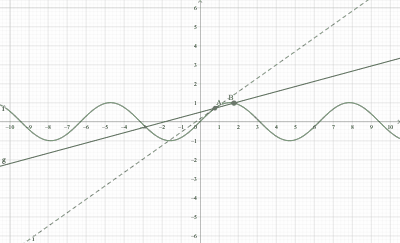
\includegraphics[width=\textwidth]{derivative.png}
      \end{center}
    \end{column}
  \end{columns}
\end{frame} 

\begin{frame}{Basic Functions and their derivatives}
  \begin{columns}
    \begin{column}{0.5\textwidth}
      \begin{block}{Basic functions}
      \begin{align*}
        \text{Polynomial}:\,f(x) &=\sum_{k=0}^n a_{k} x^{k}\\
        \text{Constant}:\, f(x) &=a\\
        \text{Expotential}:\, f(x) &= e^{x}\\
        f(x) &= a^{x}\\
        \text{Logarithmic}:\, f(x) &= \ln{(x)}\\
        \text{Trigonometric}:\, f(x) &=\sin{(x)}\\
        f(x) &=\cos{(x)}
      \end{align*}
      \end{block}
    \end{column}
    \begin{column}{0.5\textwidth}
      \begin{block}{Derivatives}
      \begin{align*}
        f'(x) &=\sum_{k=1}^{n} a_{k} k\cdot x^{(k-1)}\\
        f'(x) &=0\\
        f'(x) &=e^{x}\\
        f'(x) &=a^{x}\ln{(x)}\\
        f'(x) &=\frac{1}{x}\\
        f'(x) &=\cos{(x)}\\
        f'(x) &=-\sin{(x)}
      \end{align*}
      \end{block}
    \end{column}
  \end{columns}
\end{frame}

\begin{frame}{Properties of Derivatives}
  \begin{block}{Derivation Rules for all function $f(x)$ and $g(x)$ and all real numbers $\alpha$ and $\beta$}
    \textbf{Sum Rule}: 
    \[(\alpha f(x) +\beta g(x))'=\alpha f'(x)+\beta g'(x)\]
    \textbf{Product Rule}:
    \begin{equation}\label{eq:2}
      (f(x)g(x))'=f'(x)g(x)+f(x)g'(x) \quad \star
    \end{equation}
    \textbf{Quotient Rule}:
    \[\bigl(\frac{f(x)}{g(x)}\bigr)'=\frac{f'(x)g(x)-f(x)g'(x)}{{g(x)}^2}, \quad \text{where}\,g(x)\neq 0\]
    \textbf{Chain Rule}:
    \[(f \circ g)'(x)=f'(g(x))=f'(g(x))\cdot g'(x).\]
  \end{block}
\end{frame}

%---------------------------------------------------------------------------
\subsection{Review of Integration}
\begin{frame}{Integration}\vspace{10pt}
  \begin{block}{What is Integration}
    \textbf{Integration} can be seen as the inverse of derivation.\\
    Alternatively it is the calculation of the \textbf{area under a function}.(Thus all rules for sums apply here as well.).
  \end{block}\
  \begin{center}
    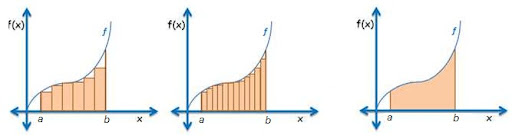
\includegraphics[height=3cm, width=10cm]{image2.png}
  \end{center}
\end{frame}

\begin{frame}{Basic Function and Their Integral}
  \begin{columns}
    \begin{column}{0.5\textwidth}
      \begin{block}{Basic Function}
        \begin{align*}
        \text{Polynomial}:\,f(x) &= x^{n}\\
        f(x) &= \frac{1}{x}\\
        \text{Constant}:\, f(x) &=a\\
        f(x) &=0\\
        \text{Expotential}:\, f(x) &= e^{x}\\
        f(x) &=a^{x}\\
        \text{Trigonometric}:\, f(x) &=\sin{(x)}\\
        f(x) &=\cos{(x)}
      \end{align*}
    \end{block}
  \end{column}
 
  \begin{column}{0.5\textwidth}
    \begin{block}{Integral}
      \begin{align*}
      F(x) &= \frac{x^{n+1}}{n+1}+C\\
      F(x) &= \ln{(\lvert x \rvert)}+C\\
      F(x) &=ax+C\\
      F(x) &=a\\
      F(x) &= e^{x}+C\\
      F(x) &= x\ln{(x)-1}\\
      F(x) &=-\cos{(x)}\\
      F(x) &= \sin{(x)}
      \end{align*}
    \end{block}
  \end{column}
\end{columns}
\end{frame}

\begin{frame}{Properties of Integration}
  \begin{block}{Integration Rules}
    \onslide<1->\textbf{Sum Rule}: 
    \[\int (f\pm g)\,\mathrm{d}x = \int f\,\mathrm{d}x\pm \int g\,\mathrm{d}x\]
    \onslide<2->\textbf{Definite Integral}: 
    \[\int_{a}^b f(x)\,\mathrm{d}x=F(b)-F(a)\]
    \onslide<3->\textbf{Substitution Rule}: 
    \[\int_{a}^{b} f(\phi(x))\phi'(x)\,\mathrm{d}x = \int_{\phi(a)}^{\phi(b)} f(u)\,\mathrm{d}x\]
    where $u=\phi(x)$.
    \end{block}
\end{frame}

\begin{frame}{Exercises}
  \onslide<1->\begin{exampleblock}{Exercise from Past Paper}
    Consider the following integral
    \[\int x\sqrt{x+4}\,\mathrm{d}x.\]
    \[\int (e^{x}+1)^{3}\,\mathrm{d}x.\]
    \[\int \cos^{3}{(x)}\cdot \sin{(x)}\,\mathrm{d}x\] %hint: hold $dx=\frac{du}{\sin{(x)}}$
  \end{exampleblock}
  \onslide<2->\begin{block}<2->{Answer}
  \[\int x \sqrt{x + 4}\,\mathrm{d}x = \frac{2}{15}(x + 4)^{3/2} (3 x - 8) + C\]
  \[\int (e^{x} + 1)^{3}\,\mathrm{d}x = x + 3 e^x + \frac{3 e^{2x}}{2} + \frac{e^{3x}}{3} + C\]
  \[\int \cos^{3}{(x)}\cdot \sin{(x)}\,\mathrm{d}x = -\frac{1}{4}\cos^{4}{(x)}+C\]
  \end{block}
\end{frame}
%---------------------------------------------------------------------------
%main presentation
\section{Formula of Integration by Parts}
\begin{frame}{An Exercise}\label{slide:1}
  \begin{tcolorbox}[enhanced,colback=red!5!white,frame style={left color=red!75!black,right color=blue!75!black},rounded corners,title=Example]
    Consider the following integral
    \[\int \ln{x}\,\mathrm{d}x.\]
    \hyperlink{slide:2}{\beamergotobutton{Verbose mode $\spadesuit$}}\\
    \pause
    \hyperlink{frame:4}{\beamerskipbutton{See Solution in \vref{frame:4}}}
  \end{tcolorbox} 
\end{frame}

\begin{frame}{Product of two Functions}\vspace{10pt}\label{slide:5}
  Given two \textit{continuous differentiable} function $f(x)$ and $g(x)$, and product rule states:
  \[(fg)'=f'g+fg'.\]
  integrating both sides with respect to $x$,
  \[\int (fg)'(x)\,\mathrm{d}x = \int f'(x)\cdot g(x)\,\mathrm{d}x + \int f(x)\cdot g'(x)\,\mathrm{d}x\]
  \[\Longrightarrow \quad f(x)\cdot g(x)= \int f'(x)\cdot g(x)\,\mathrm{d}x + \int f(x)\cdot g'(x)\,\mathrm{d}x\]
  \[\Longrightarrow \quad \int \textcolor[rgb]{1,0,1}{f'(x)}\cdot \textcolor[rgb]{0.77,0.12,0.23}{g(x)}\,\mathrm{d}x = \textcolor[rgb]{1,0,1}{f(x)}\cdot \textcolor[rgb]{0.77,0.12,0.23}{g(x)} - \int \textcolor[rgb]{1,0,1}{f(x)}\cdot \textcolor[rgb]{0.77,0.12,0.23}{g'(x)}\,\mathrm{d}x\]
  This yields the formula for definte integral:\vspace{-2mm}
  \begin{tcolorbox}[enhanced,colframe=red!75!black,interior style={left color=red!20!white,right color=yellow!50!white},rounded corners]
    \begin{equation}\label{partielle integration}
      \int_a^b \textcolor[rgb]{1,0,1}{f'(x)} \cdot \textcolor[rgb]{0.77,0.12,0.23}{g(x)}\,\mathrm{d}x = \Bigl. \textcolor[rgb]{1,0,1}{f(x)} \cdot \textcolor[rgb]{0.77,0.12,0.23}{g(x)}\Bigr|_a^{b} - \int_a^b \textcolor[rgb]{1,0,1}{f(x)} \cdot \textcolor[rgb]{0.77,0.12,0.23}{g'(x)}\,\mathrm{d}x.
    \end{equation}
  \end{tcolorbox}
\end{frame}
%I have finished my work at here. 15.Aug.
\begin{frame}{Answer of Question in \vref{slide:1}}\vspace{10pt}\label{frame:4}
  We choose $f'(x)=1$ and $g(x)=\ln{(x)}$ in \Cref{partielle integration}, so we get $f(x)=x$ and $g'(x)=\frac{1}{x}$:
  \begin{align*}
    \int \underbrace{\textcolor[rgb]{1,0,1}{1} \cdot \textcolor[rgb]{0.77,0.12,0.23}{\ln{(x)}}}_{\textcolor[rgb]{1,0,1}{f'(x)} \cdot \textcolor[rgb]{0.77,0.12,0.23}{g(x)}}\,\mathrm{d}x 
    &=\underbrace{\textcolor[rgb]{1,0,1}{x}\cdot \textcolor[rgb]{0.77,0.12,0.23}{\ln{(x)}}}_{\textcolor[rgb]{1,0,1}{f(x)}\cdot \textcolor[rgb]{0.77,0.12,0.23}{g(x)}} - \int \underbrace{\textcolor[rgb]{1,0,1}{x}\cdot \textcolor[rgb]{0.77,0.12,0.23}{\frac{1}{x}}}_{\textcolor[rgb]{1,0,1}{f(x)}\cdot \textcolor[rgb]{0.77,0.12,0.23}{g'(x)}}\,\mathrm{d}x\\
    &=x\ln{(x)} - x + C.
  \end{align*}
\end{frame}

\begin{frame}{Calculation of Integrals through Trick:LIATE Rule}
  \begin{tcolorbox}[enhanced,colback=red!5!white,frame style={left color=red!75!black,right color=blue!75!black},
    sharp corners=uphill,arc=6mm,boxrule=2mm,boxsep=5mm,title=Choosing $g(x)$ that comes first in the following list]
    \begin{enumerate}
      \item \textbf{L}: logarithmic function\\
      \item \textbf{I}: inverse trigonometric function\\
      \item \textbf{A}: algebraic function (e.g. $x^3, 3x^{50}$)\\
      \item \textbf{T}: trigonometric function\\
      \item \textbf{E}: expotential function
    \end{enumerate}
  \end{tcolorbox}
\end{frame}

\begin{frame}{Calculation of Integrals through Trick:LIATE Rule}\label{slide:6}
  \begin{tcolorbox}[enhanced,frame style image=blueshade.png,
    opacityback=0.75,opacitybacktitle=0.25,
    colback=blue!5!white,colframe=blue!75!black,
    title=Exercises]
    \begin{enumerate}
      \item \begin{equation}\label{qe:1}
        \int_{0}^{\pi} \sin{(x)}\cdot x\,\mathrm{d}x
      \end{equation}
      \pause
      \hfill 
      \hyperlink{slide:7}{\beamergotobutton{See Solution in \vref{slide:7}}}\\
      \pause
      \item \begin{equation}\label{qe:2}
        \int e^{x}\cdot (2-x^2)\,\mathrm{d}x
      \end{equation}
      \pause
      \hfill
      \hyperlink{slide:8}{\beamergotobutton{See Solution in \vref{slide:8}}}\\
      \pause
      \item \begin{equation}\label{qe:3}
        \int x^3 e^{x^{2}}\,\mathrm{d}x
      \end{equation}
      \pause
      \hfill
      \hyperlink{slide:9}{\beamergotobutton{See Solution in \vref{slide:9}}}
    \end{enumerate}
  \end{tcolorbox}
\end{frame}

\begin{frame}{Answer of \Cref{qe:1}}\vspace{4pt}\label{slide:7}
  We choose $f'(x)=\sin{(x)}$ and $g(x)=x$ in \Cref{partielle integration}, 
  so that we get $f(x)=-\cos{(x)}$ and $g'(x)=1$:
  \begin{align*}
    \int_0^{\pi} \underbrace{\textcolor[rgb]{1,0,1}{\sin{(x)}} \cdot \textcolor[rgb]{0.77,0.12,0.23}{x}}_{\textcolor[rgb]{1,0,1}{f'(x)}\cdot \textcolor[rgb]{0.77,0.12,0.23}{g(x)}}\,\mathrm{d}x 
    &= \Bigl. \underbrace{\textcolor[rgb]{1,0,1}{-\cos{(x)}} \cdot \textcolor[rgb]{0.77,0.12,0.23}{x}}_{\textcolor[rgb]{1,0,1}{f'(x)}\cdot \textcolor[rgb]{0.77,0.12,0.23}{g(x)}}\Bigr|_0^{\pi} 
    - \int_0^{\pi} \underbrace{\textcolor[rgb]{1,0,1}{(-\cos{(x)})}\cdot \textcolor[rgb]{0.77,0.12,0.23}{1}}_{\textcolor[rgb]{1,0,1}{f'(x)}\cdot \textcolor[rgb]{0.77,0.12,0.23}{g(x)}}\,\mathrm{d}x\\
    &= \Bigl. -\cos{(x)}\cdot x\Bigr|_{0}^{\pi} + \int_0^{\pi} \cos{(x)}\,\mathrm{d}x\\
    &= \Bigl. -\cos{(x)}\cdot x\Bigr|_{0}^{\pi} + \Bigl. \sin{(x)}\Bigr|_{0}^{\pi}\\
    &= -\pi \cos{(\pi)} + 0 \cdot \cos{(0)} + \sin{(\pi)} - \sin{(0)}\\
    &= -\pi \cdot (-1)\\
    &= \pi
  \end{align*}
  \vspace{4pt}
  \hyperlink{qe:2}{\beamerreturnbutton{Return $\clubsuit$}}
\end{frame}

\begin{frame}{Answer of \Cref{qe:2}}\label{slide:8}
  We choose $f'(x)=e^{x}$ and $g(x)$ as the remaining polynomial term in \Cref{partielle integration},
  so that we get:
  \begin{align*}
    \int \underbrace{\textcolor[rgb]{1,0,1}{e^{x}}\cdot \textcolor[rgb]{0.77,0.12,0.23}{(2-x^2)}}_{\textcolor[rgb]{1,0,1}{f'(x)}\cdot \textcolor[rgb]{0.77,0.12,0.23}{g(x)}}\,\mathrm{d}x
    &= \underbrace{\textcolor[rgb]{1,0,1}{e^{x}}\cdot \textcolor[rgb]{0.77,0.12,0.23}{(2-x^2)}}_{\textcolor[rgb]{1,0,1}{f(x)}\cdot \textcolor[rgb]{0.77,0.12,0.23}{g(x)}}
    -\int \underbrace{\textcolor[rgb]{1,0,1}{e^{x}}\cdot \textcolor[rgb]{0.77,0.12,0.23}{(-2x)}}_{\textcolor[rgb]{1,0,1}{f(x)}\cdot \textcolor[rgb]{0.77,0.12,0.23}{g'(x)}}\,\mathrm{d}x\\
    &= e^x \cdot (2-x^2) + \int \underbrace{\textcolor[rgb]{1,0,1}{e^{x}}\cdot \textcolor[rgb]{0.77,0.12,0.23}{2x}}_{\textcolor[rgb]{1,0,1}{f'(x)}\cdot \textcolor[rgb]{0.77,0.12,0.23}{g(x)}}\,\mathrm{d}x\\
    &= e^x \cdot (2-x^2) + \Biggl(\underbrace{\textcolor[rgb]{1,0,1}{e^{x}}\cdot \textcolor[rgb]{0.77,0.12,0.23}{(2x)}}_{\textcolor[rgb]{1,0,1}{f'(x)}\cdot \textcolor[rgb]{0.77,0.12,0.23}{g(x)}}
    -\int \underbrace{\textcolor[rgb]{1,0,1}{e^{x}}\cdot \textcolor[rgb]{0.77,0.12,0.23}{2}}_{\textcolor[rgb]{1,0,1}{f(x)}\cdot \textcolor[rgb]{0.77,0.12,0.23}{g'(x)}}\,\mathrm{d}x\Biggr)\\
    &= e^x \cdot (2-x^2) + e^x \cdot 2x - 2 \cdot e^x + C\\
    &= e^x (2x-x^2)+C
  \end{align*}
  \vspace{4pt}
  \hyperlink{slide:6}{\beamerreturnbutton{Return $\clubsuit$}}
\end{frame}

\begin{frame}{Answer of \Cref{qe:3}}\vspace{4pt}\label{slide:9}
  We choose $f'(x)=x \cdot e^{x^{2}}$ and $g(x)=x^2$ in \Cref{partielle integration}, 
  so that we get $f(x) = \frac{e^{x^{2}}}{2}$ and $g'(x)= 2x$:
  \begin{align*}
    \int \underbrace{\textcolor[rgb]{1,0,1}{(x e^{x^{2}})}\cdot \textcolor[rgb]{0.77,0.12,0.23}{(x^2)}}_{\textcolor[rgb]{1,0,1}{f'(x)}\cdot \textcolor[rgb]{0.77,0.12,0.23}{g(x)}}\,\mathrm{d}x
    &= \underbrace{\textcolor[rgb]{1,0,1}{\frac{e^{x^{2}}}{2}}\cdot \textcolor[rgb]{0.77,0.12,0.23}{x^2}}_{\textcolor[rgb]{1,0,1}{f(x)}\cdot \textcolor[rgb]{0.77,0.12,0.23}{g(x)}}
    - \int \underbrace{\textcolor[rgb]{1,0,1}{\frac{e^{x^{2}}}{2}}\cdot \textcolor[rgb]{0.77,0.12,0.23}{2x}}_{\textcolor[rgb]{1,0,1}{f(x)}\cdot \textcolor[rgb]{0.77,0.12,0.23}{g'(x)}}\,\mathrm{d}x\\
    &= \frac{x^{2}e^{x^{2}}}{2} - \int x\cdot e^{x^{2}}\,\mathrm{d}x\\
    &= \frac{x^{2}e^{x^{2}}}{2} - \frac{e^{x^{2}}}{2} + C\\
    &= \frac{e^{x^{2}}(x^{2}-1)}{2} + C
  \end{align*}
  \vspace{4pt}
  \hyperlink{slide:6}{\beamerreturnbutton{Return $\clubsuit$}}
\end{frame}

\begin{frame}{Indirect Calculation of Integrals by \Cref{partielle integration}}\vspace{10pt}\label{slide:10}
  \begin{tcolorbox}[enhanced,colback=red!5!white,frame style={left color=red!75!black,right color=blue!75!black},rounded corners,title=Exercise]
    Consider the following integral:
    \begin{equation}\label{qe:4}
      \int \sin{(x)}\cdot \cos{(x)}\,\mathrm{d}x
    \end{equation}
    \pause
    \hfill
    \hyperlink{slide:11}{\beamergotobutton{See Solution in \vref{qe:4}}}
  \end{tcolorbox}
\end{frame}

\begin{frame}{Answer of \Cref{qe:4}}\vspace{10pt}\label{slide:11}
  We choose $f'(x)=\sin{(x)}$ and $g(x)=\cos{(x)}$ in \Cref{partielle integration},
  so that we get $f(x)=-\cos{(x)}$ and $g'(x)=-\sin{(x)}$:
  \begin{align*}
    \int \underbrace{\textcolor[rgb]{1,0,1}{\sin{(x)}}\cdot \textcolor[rgb]{0.77,0.12,0.23}{\cos{(x)}}}_{\textcolor[rgb]{1,0,1}{f'(x)}\cdot \textcolor[rgb]{0.77,0.12,0.23}{g(x)}}\,\mathrm{d}x
    &= \underbrace{\textcolor[rgb]{1,0,1}{-\cos{(x)}}\cdot \textcolor[rgb]{0.77,0.12,0.23}{\cos{(x)}}}_{\textcolor[rgb]{1,0,1}{f(x)}\cdot \textcolor[rgb]{0.77,0.12,0.23}{g(x)}} 
    - \int \underbrace{\textcolor[rgb]{1,0,1}{(-\cos{(x)})}\cdot \textcolor[rgb]{0.77,0.12,0.23}{(-\sin{(x)})}}_{\textcolor[rgb]{1,0,1}{f(x)}\cdot \textcolor[rgb]{0.77,0.12,0.23}{g'(x)}}\,\mathrm{d}x\\
    &= -\cos^2{(x)} - \int \cos{(x)}\cdot \sin{(x)}\,\mathrm{d}x 
  \end{align*}
  We add up both side of equation the integral $\int \cos{(x)}\cdot \sin{(x)}\,\mathrm{d}x$, so we get 
  \[2 \int \cos{(x)}\cdot \sin{(x)}\,\mathrm{d}x = -\cos^2{(x)}\]
  \[\Longrightarrow \int \cos{(x)}\cdot \sin{(x)}\,\mathrm{d}x = -\frac{1}{2}\cos^2{(x)} + C.\]
  \vspace{10pt}
  \hyperlink{slide:10}{\beamerreturnbutton{Return $\clubsuit$}}
\end{frame}

\begin{frame}{Calculation of Recursion Formula by \Cref{partielle integration}}\vspace{10pt}\label{slide:12}
  \begin{tcolorbox}[enhanced,colback=red!5!white,frame style={left color=red!75!black,right color=blue!75!black},rounded corners,title=Example]
    Given the following integral,
    \[\int \sin^{n}{(x)}\,\mathrm{d}x,\]
    where $n$ is integer, prove the following recursion formula:
    \begin{equation}\label{qe:5}
      \int \sin^{n}{(x)}\,\mathrm{d}x = -\frac{1}{n}\cos{(x)}\cdot \sin^{n-1}{(x)} 
      +\frac{n-1}{n}\int \sin^{n-2}{(x)}\,\mathrm{d}x
    \end{equation}
    \pause 
    \hfill
    \hyperlink{slide:13}{\beamergotobutton{See Solution in \vref{qe:5}}}
  \end{tcolorbox}
\end{frame}

\begin{frame}{Answer of \Cref{qe:5}}\vspace{4pt}\label{slide:13}
    \begin{align*}
      \int \sin^n{(x)}\,\mathrm{d}x &= \int \sin{(x)}\cdot \sin^{n-1}{(x)}\,\mathrm{d}x\\
      &\textcolor[rgb]{0.0,0.5,0.0}{\downarrow \text{Choose}\,f'(x)= \sin{(x)}\, \text{and}\, g(x)= \sin^{n-1}{(x)}}\\ 
      &\qquad \textcolor[rgb]{0.0,0.5,0.0}{\Longrightarrow f(x)= -\cos{(x)} \text{and}\, g'(x)=(n-1)\sin^{n-2}{(x)}\cos{(x)}}\\
      &= \underbrace{-\cos{(x)}\cdot \sin^{n-1}{(x)}}_{f(x)\cdot g(x)} - \int \underbrace{(-\cos{(x)})\cdot (n-1)\sin^{n-2}{(x)}\cos{(x)}}_{f(x)\cdot g(x)}\,\mathrm{d}x\\
      &= -\cos{(x)}\cdot \sin^{n-1}{(x)} + (n-1)\int \cos^2{(x)}\sin^{n-2}{(x)}\,\mathrm{d}x
    \end{align*}
    We would like to make the integral in the right side in the form $\int \sin^m{(x)}\,\mathrm{d}x$ with $m \leq n$,
    so that we use Pythagorean trigonometric identity,
    \[\sin^2{(x)}+\cos^2{(x)}=1 \quad \Longrightarrow \cos^{(x)} = 1- \sin^2{(x)}\]
    and we get 
    \hfill
    \hyperlink{slide:14}{\beamergotobutton{Next $\blacksquare$}}
\end{frame}

\begin{frame}{Cont. Answer of \Cref{qe:5}}\vspace{4pt}\label{slide:14}
  \begin{align*}
  \int \sin^n{(x)}\,\mathrm{d}x &= -\cos{(x)}\cdot \sin^{n-1}{(x)} + (n-1)\int \cos^2{(x)}\sin^{n-2}{(x)}\,\mathrm{d}x\\
  &\textcolor[rgb]{0.0,0.5,0.0}{\downarrow \text{Pythagorean identity}}\\
  &= -\cos{(x)}\cdot \sin^{n-1}{(x)} + (n-1)\int (1-\sin^2{(x)})\sin^{n-2}{(x)}\,\mathrm{d}x\\
  &= -\cos{(x)}\cdot \sin^{n-1}{(x)} + (n-1)\int \sin^{n-2}{(x)}\,\mathrm{d}x - (n-1)\int \sin^n{(x)}\,\mathrm{d}x\\
  \end{align*}
  We add up both side of equation the integral $(n-1)\int \sin^n{(x)}\,\mathrm{d}x$, so we get 
  \[n \int \sin^n{(x)}\,\mathrm{d}x = -\cos{(x)}\cdot \sin^{n-1}{(x)} + (n-1)\int \sin^{n-2}{(x)}\,\mathrm{d}x.\]
  We get the recursion formula through dividing the both side of equation by $n$
  \[\int \sin^{n}{(x)}\,\mathrm{d}x = -\frac{1}{n}\cos{(x)}\cdot \sin^{n-1}{(x)} 
  +\frac{n-1}{n}\int \sin^{n-2}{(x)}\,\mathrm{d}x\]
  \hfill
  \hyperlink{slide:12}{\beamerreturnbutton{Return $\clubsuit$}}
\end{frame}

\begin{frame}{Integration by Parts}\vspace{4pt}
  \begin{center}
    
\includegraphics[width=0.7\textwidth]{image3.png}
  \end{center}
\end{frame}
%--------------------------------------------------------------------------------------
\appendix
 \begin{frame}{Basic Function and Their Integral}\label{slide:2}
  \begin{columns}
    \begin{column}{0.5\textwidth}
      \begin{block}{Basic Function \hfill \hyperlink{slide:5}{\beamergotobutton{Return $\blacksquare$}}}
        \begin{align*}
          \text{Polynomial}:\,f(x) &= x^{n}\\
          f(x) &= \frac{1}{x}\\
          \text{Constant}:\, f(x) &=a\\
          f(x) &=0\\
          \text{Expotential}:\, f(x) &= e^{x}\\
          f(x) &=a^{x}\\
          \text{Trigonometric}:\, f(x) &=\sin{(x)}\\
          f(x) &=\cos{(x)}
        \end{align*}
      \end{block}
    \end{column}
 
    \begin{column}{0.5\textwidth}
      \begin{block}{Integral \hfill \hyperlink{slide:3}{\beamergotobutton{Next $\clubsuit$}}}
        \begin{align*}
          F(x) &= \frac{x^{n+1}}{n+1}+C\\
          F(x) &= \ln{(\lvert x \rvert)}+C\\
          F(x) &=ax+C\\
          F(x) &=a\\
          F(x) &= e^{x}+C\\
          F(x) &= x\ln{(x)-1}\\
          F(x) &=-\cos{(x)}\\
          F(x) &= \sin{(x)}
        \end{align*}
      \end{block}
    \end{column}
  \end{columns}
\end{frame}

\begin{frame}{Properties of Integration}\label{slide:3}
  \begin{block}{Integration Rules}
    \textbf{Sum Rule}: 
    \[\int (f\pm g)\,\mathrm{d}x = \int f\,\mathrm{d}x\pm \int g\,\mathrm{d}x\]
    \textbf{Definite Integral}: 
    \[\int_{a}^b f(x)\,\mathrm{d}x=F(b)-F(a)\]
    \textbf{Substitution Rule}: 
    \[\int_{a}^{b} f(\psi(x))\psi'(x)\,\mathrm{d}x = \int_{\psi(a)}^{\psi(b)} f(u)\,\mathrm{d}x\]
    where $u=\psi(x)$.
  \end{block}
  \begin{tcolorbox}[width=\linewidth,sharp corners=downhill,arc=3mm,boxrule=1mm,
    colback=white,colframe=cyan,
    title style={left color=black,right color=cyan},halign=center,valign=center,sidebyside]
    \hyperlink{slide:5}{\beamerreturnbutton{Return $\blacksquare$}}
    \tcblower
    \hyperlink{slide:1}{\beamerreturnbutton{Return $\clubsuit$}}
  \end{tcolorbox}
\end{frame}
\end{document}